\section{Rethinking storage model for Docker registry}
\label{sec:file_adressable}

%\subsection{}
\paragraph{Benefit of file-level content addressable storage}
Docker registry can save a lot of space if using file-level content addressable storage. 
Benefit: saving money, reducing storage management overhead.

\subsection{Two file-level content addressable storage models}

\begin{figure}
	\centering
	%\includegraphics [width=0.45\textwidth]{plots/exp-total-stev-erase.eps}
	\subfigure[Recompression layers]{\label{fig:per_layer_ratio_fcnt_cdf}
		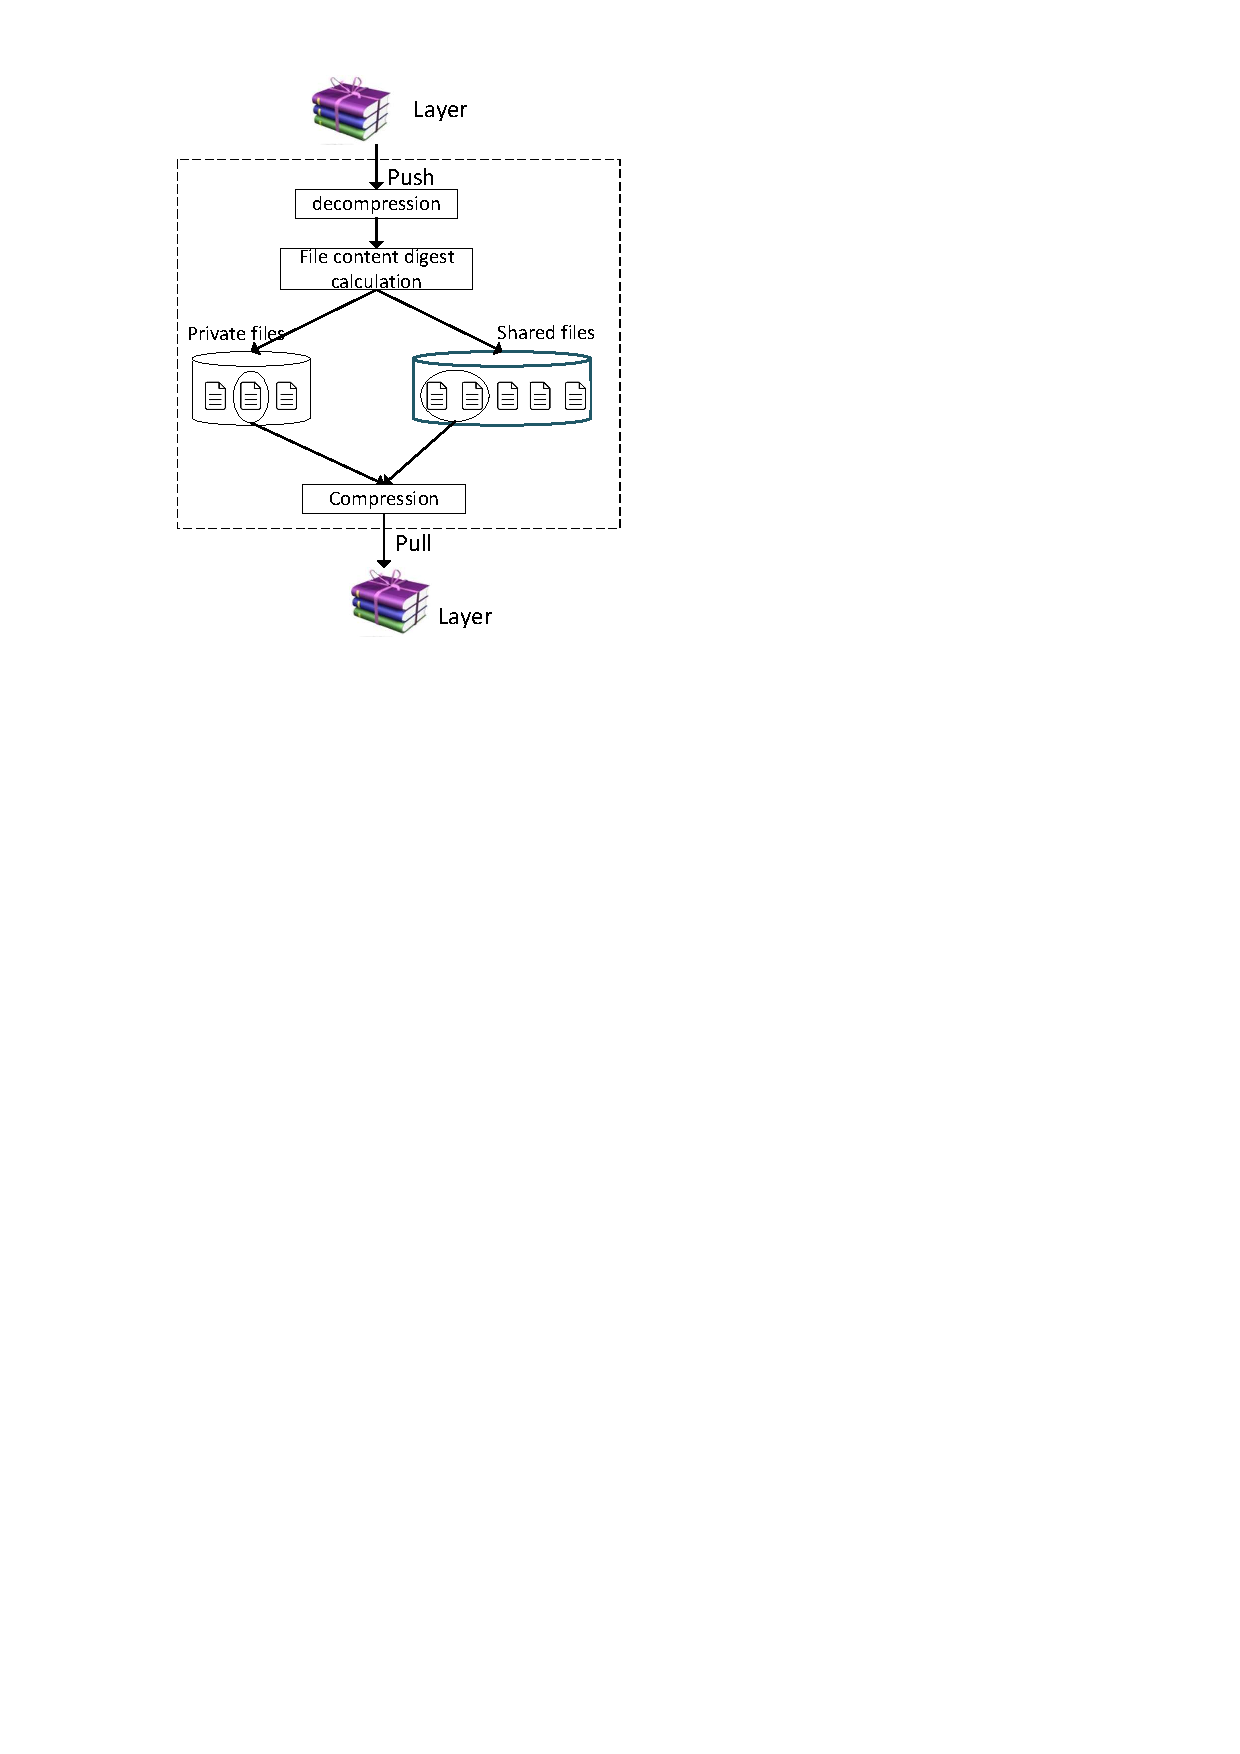
\includegraphics [width=0.21\textwidth]{graphs/graph_compression_layers.pdf}
	}
	\subfigure[Reconstruct layers]{\label{fig:per_layer_ratio_fcnt_pdf}
		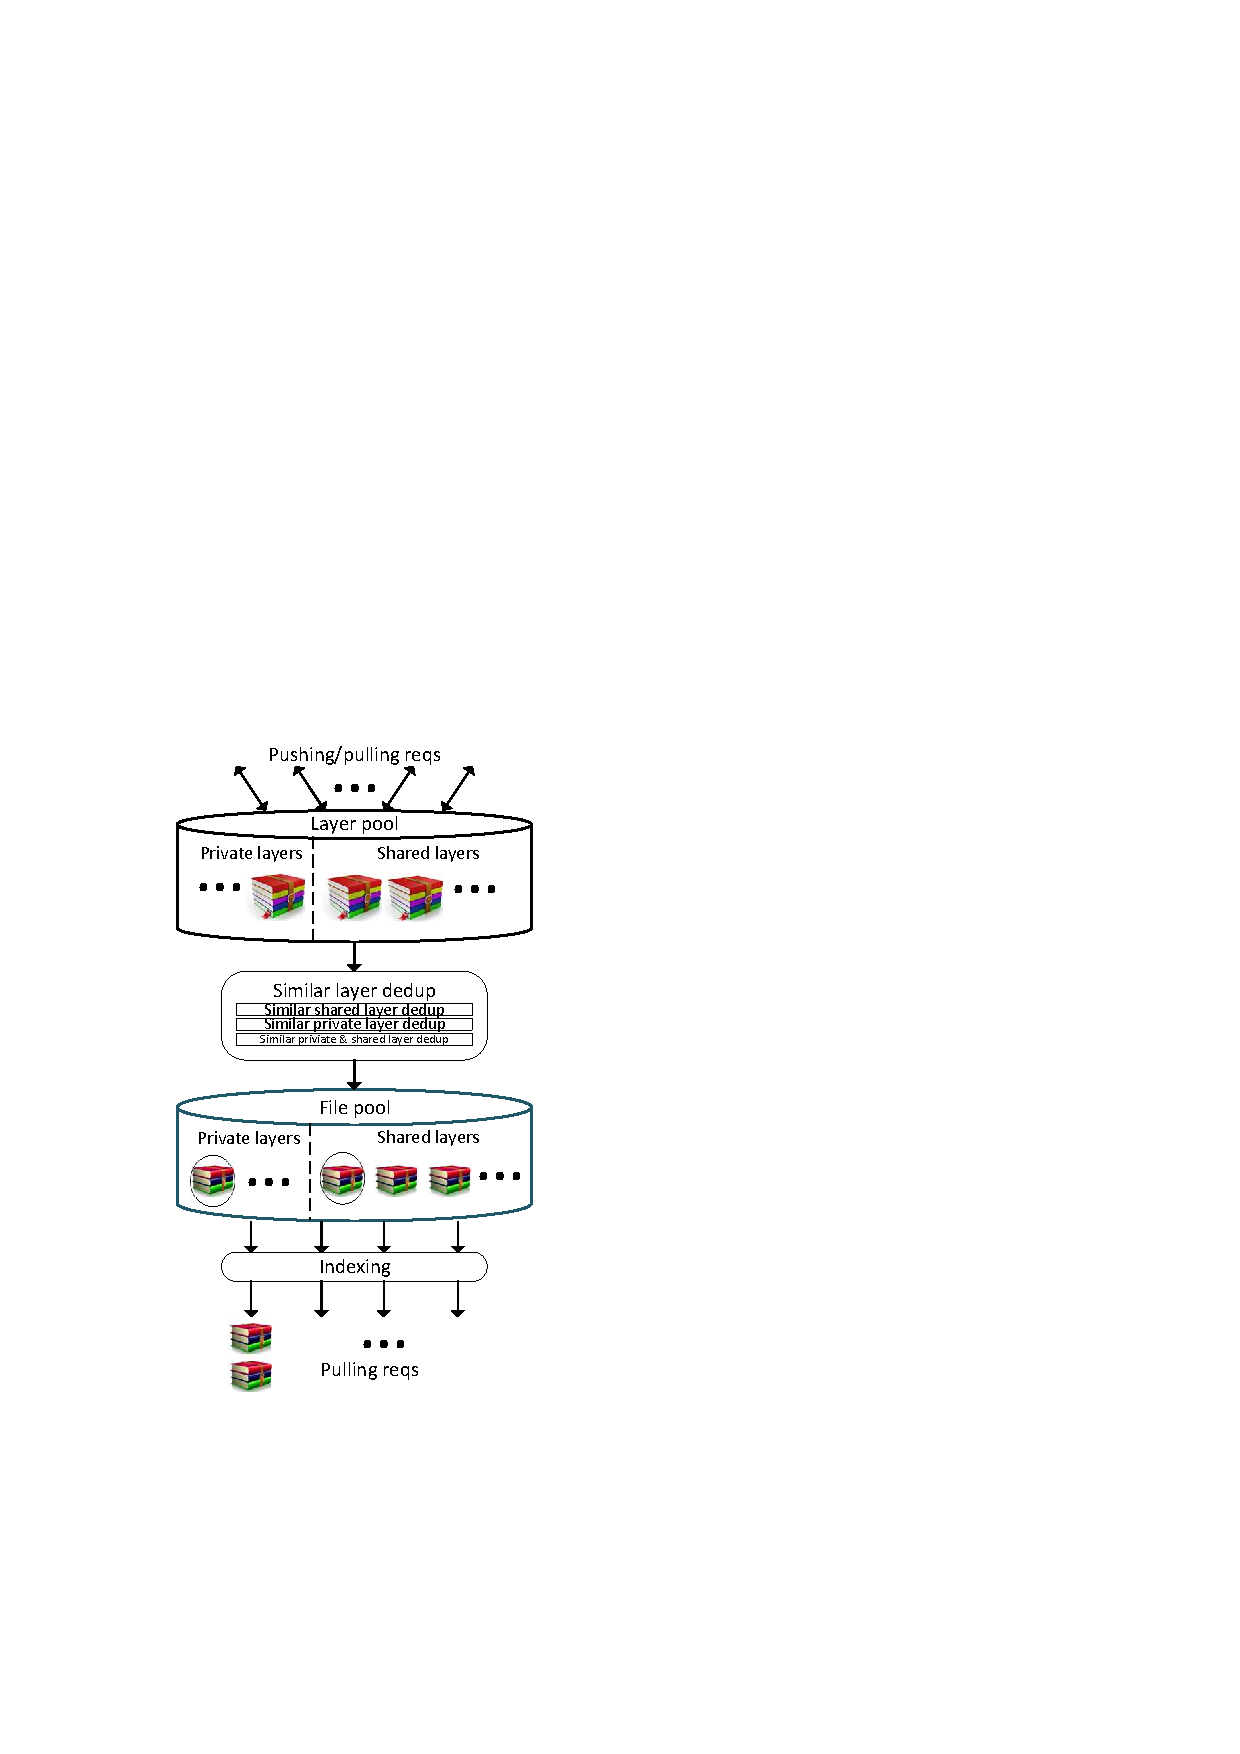
\includegraphics [width=0.24\textwidth]{graphs/graph_reconstruct_layers.pdf}
	}
	\caption{File-level content addressable storage model}
	\label{fig:eval-stdev-erasure-cnt}
\end{figure}

\subsection{Hints for performance improvement and storage saving}

\begin{table} 
	\centering 
	\scriptsize  
	%\begin{minipage}{.5\linewidth}
	\caption{Latency breakdown} \label{tbl:redundant_ratio} 
	\begin{tabular}{|l|l|l|l|l|}%p{0.14\textwidth} 
		\hline 
		% after \\: \hline or \cline{col1-col2} \cline{col3-col4} ... 
		% after \\: \hline or \cline{col1-col2} \cline{col3-col4} ... 
		Operations/latency (S) & max & min & median & avg.\\
		\hline
		 gunzip decompression (RAM) &   &   &    &  \\
 		\hline
 		tar extraction (RAM) &   &   &    &  \\
		\hline
		Digest calculation (RAM) &  &  & & \\
		\hline
		tar archiving (RAM)  &  &  & &\\
		\hline
		gzip compression (RAM) & &  &  & \\
		\hline
		Total time (RAM) (with compression) & & & & \\
		\hline
		Total time (RAM) (without compression) & & & & \\
		\hline
 		\hline
 		gunzip decompression (SSD) &   &   &    &  \\
 		\hline
 		tar extraction (SSD) &   &   &    &  \\
		\hline
		Digest calculation (SSD) &  &  & & \\
		\hline
		tar archiving (SSD) &  &  & & \\
		\hline
		gzip compression (SSD) & &  &  & \\
		\hline		 
		Total time (SSD) (with compression) & & & & \\
		\hline
		Total time (SSD) (without compression) & & & & \\
		\hline
		\hline
		Network transfer & & & & \\
		\hline 	
	\end{tabular} 
\end{table} 

\subsubsection{Compression or Archiving?} 

\paragraph{CDF and PDF of latencies} 

Compression time during pulling. 

\paragraph{Small compression ratio and small layer size}

\begin{figure}[!t]
	\centering
	\subfigure[CDF of compression ratio]{\label{fig_cdf_compression_ratio}
		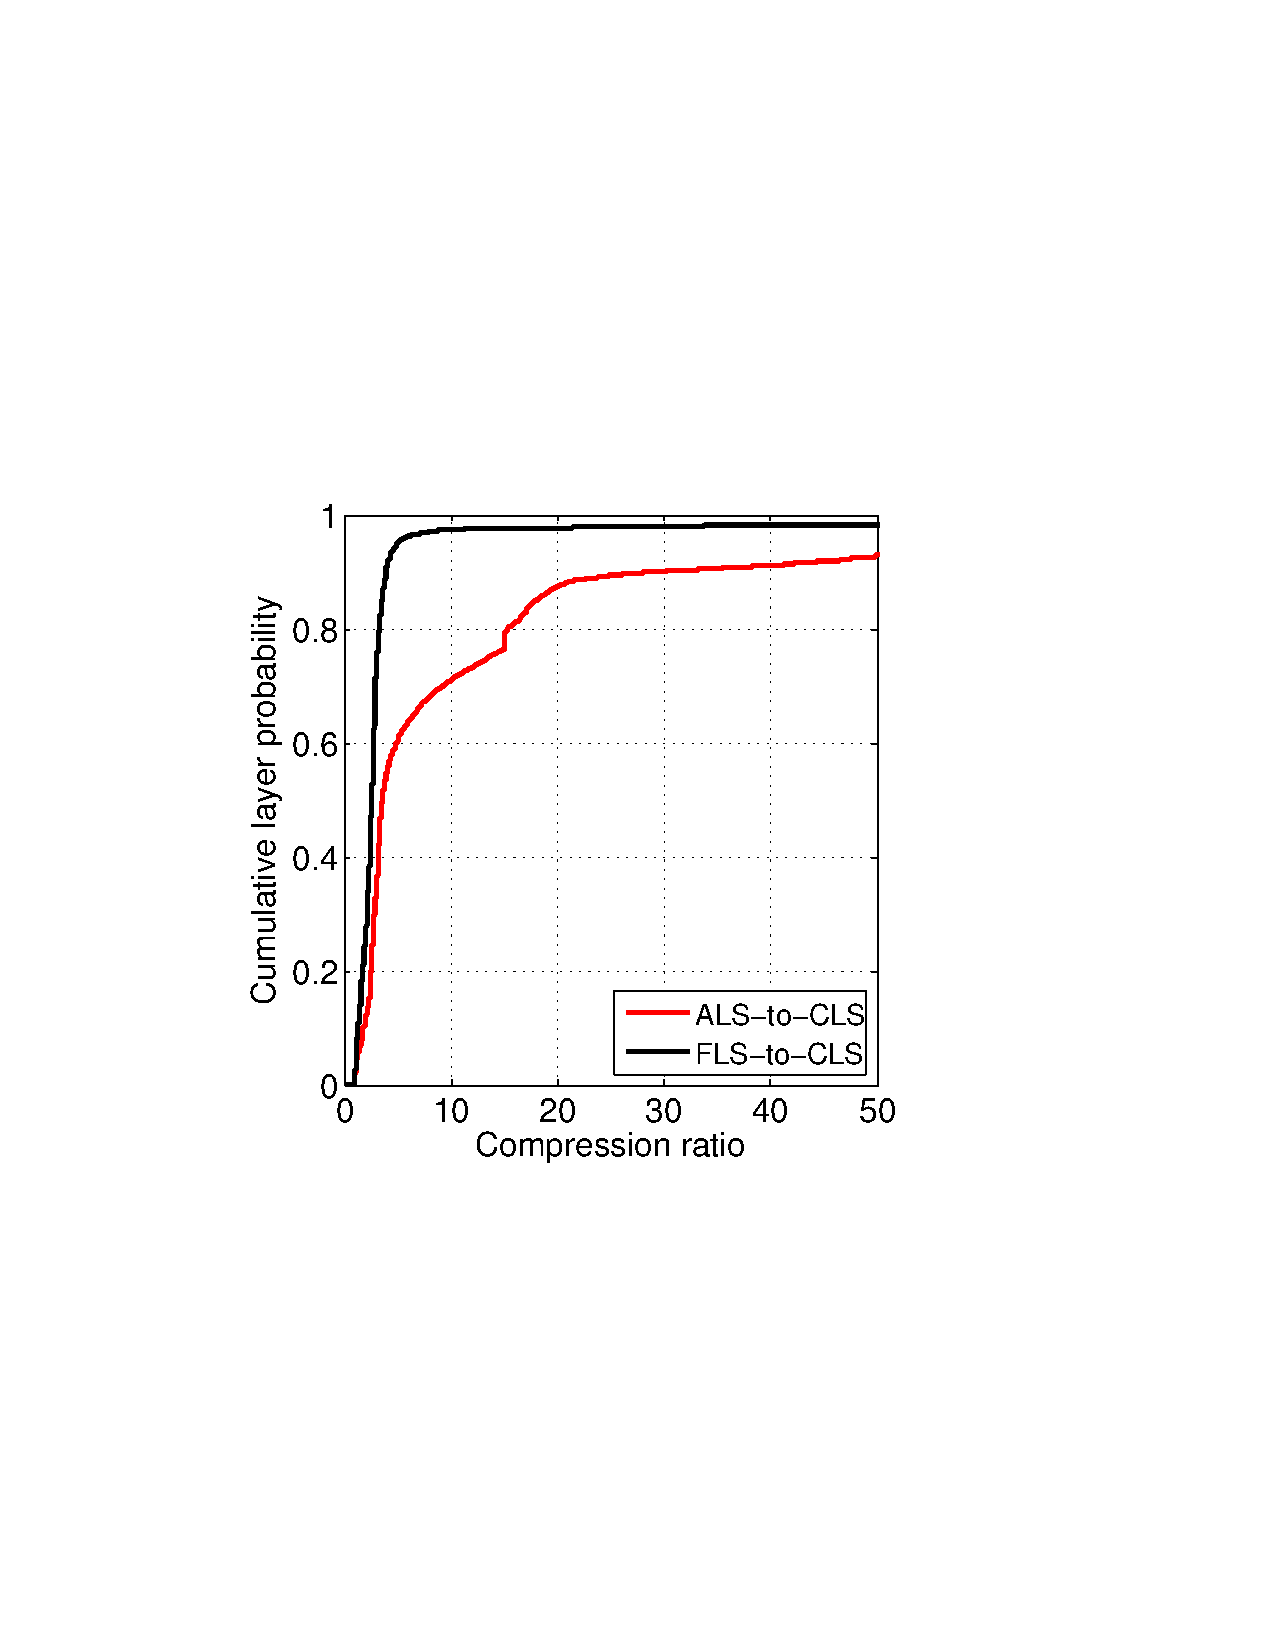
\includegraphics[width=0.23\textwidth]{graphs/cdf_compression_ratio.pdf}
	}
	\subfigure[Histogram of comp. ratios]{\label{fig_his_compression_ratio}
		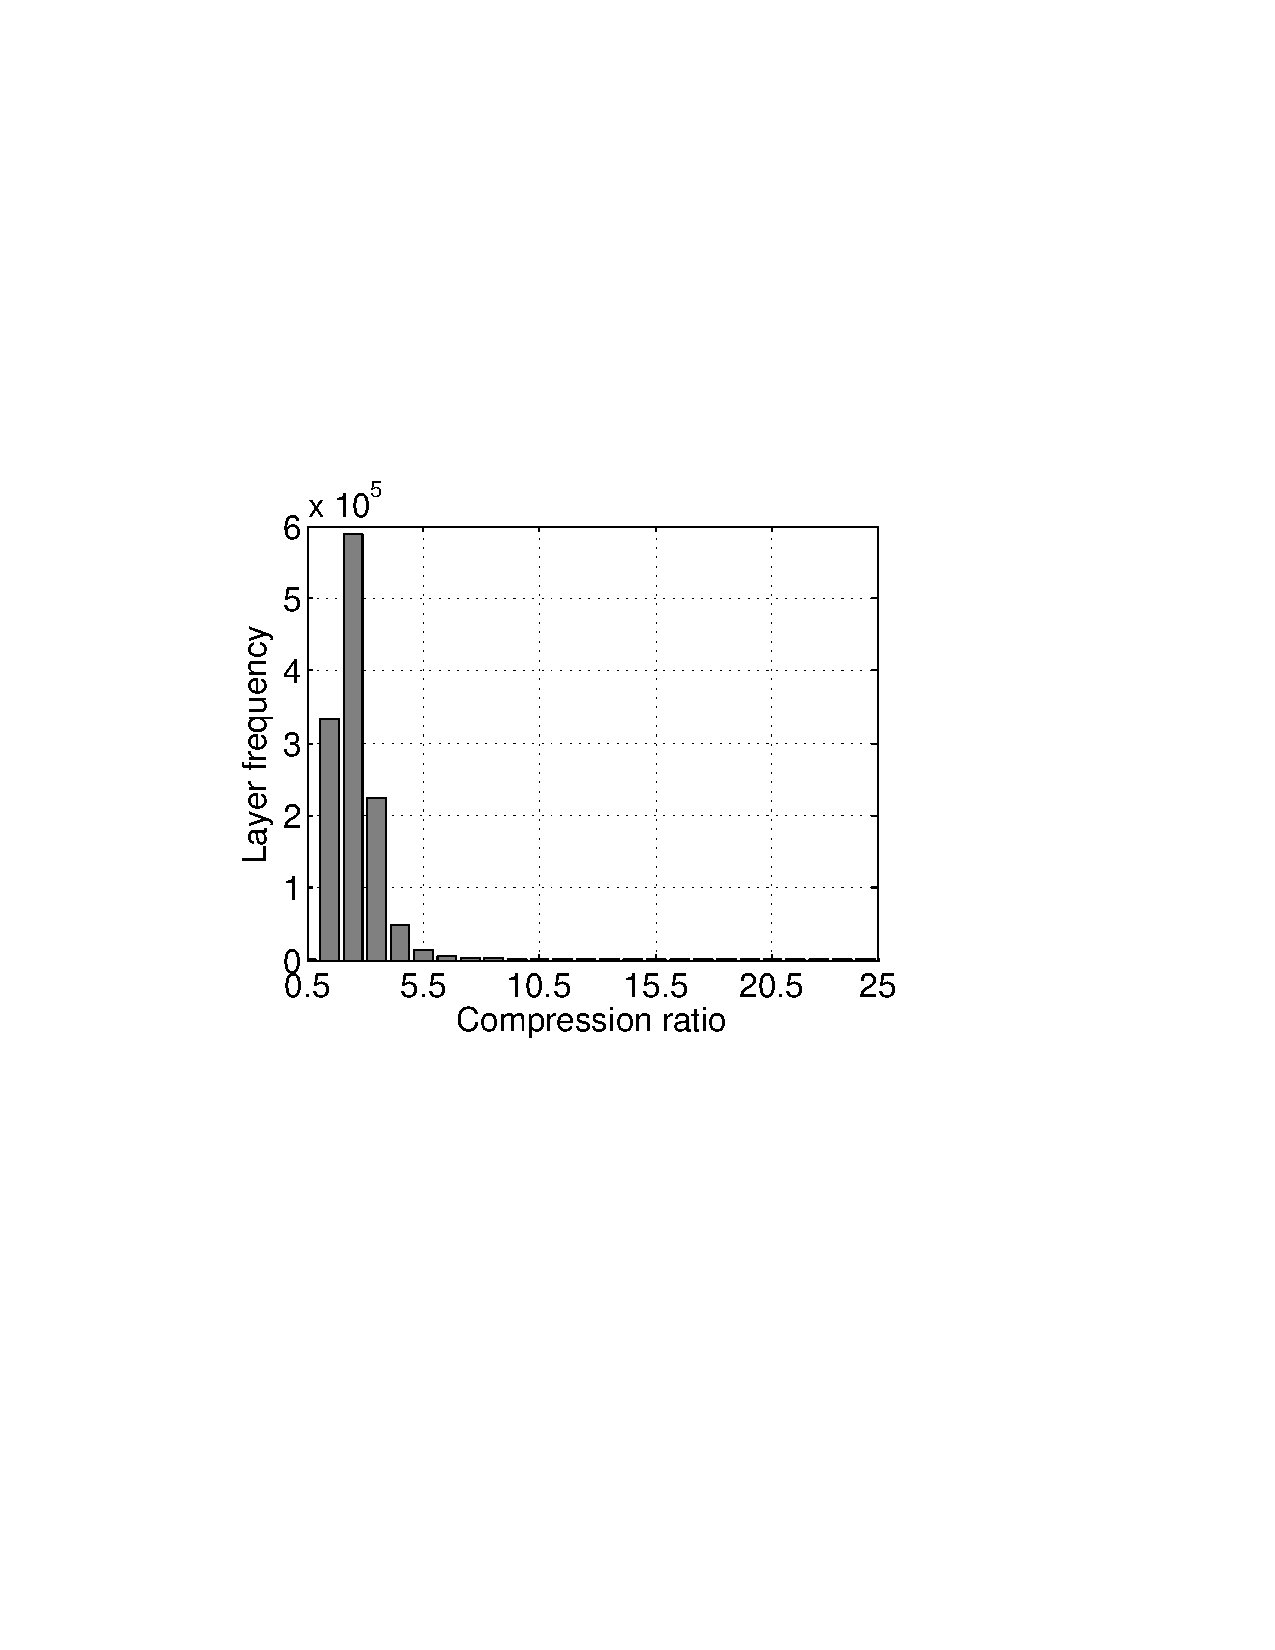
\includegraphics[width=0.223\textwidth]{graphs/his_compression_ratio.pdf}
	}
	\caption{Layer compression ratio distribution
	%\vcomment{Different colors are used in figure (a) and (b) FLS/CLS\nancomment{will address later}}
	}
	\label{fig-compression-ratio}
\end{figure}


\begin{figure}[!t]
	\centering
	\subfigure[CDF of layer sizes]{\label{fig_layer_size_cdf}
		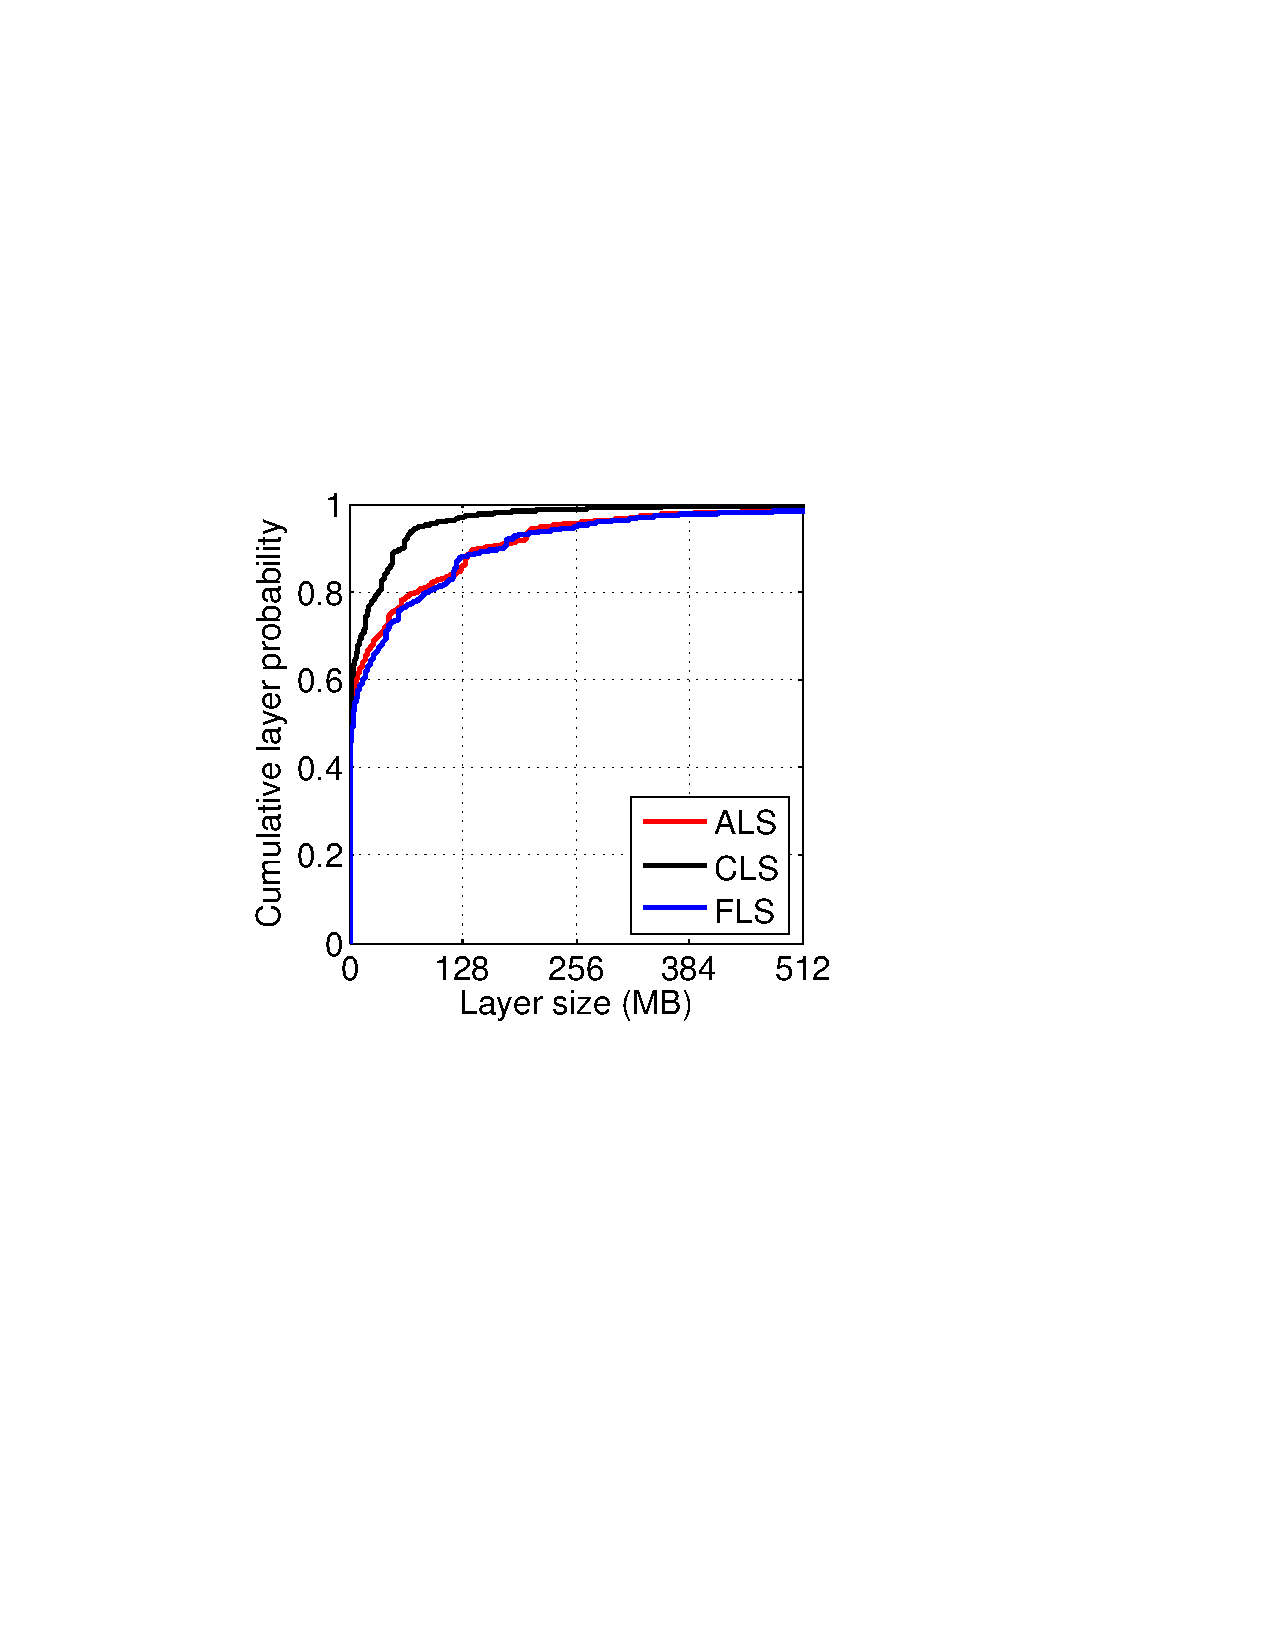
\includegraphics[width=0.234\textwidth]{graphs/layer_size_mb.pdf}
	}
	\subfigure[Histogram of layer sizes]{\label{fig_hist_layer_size}
		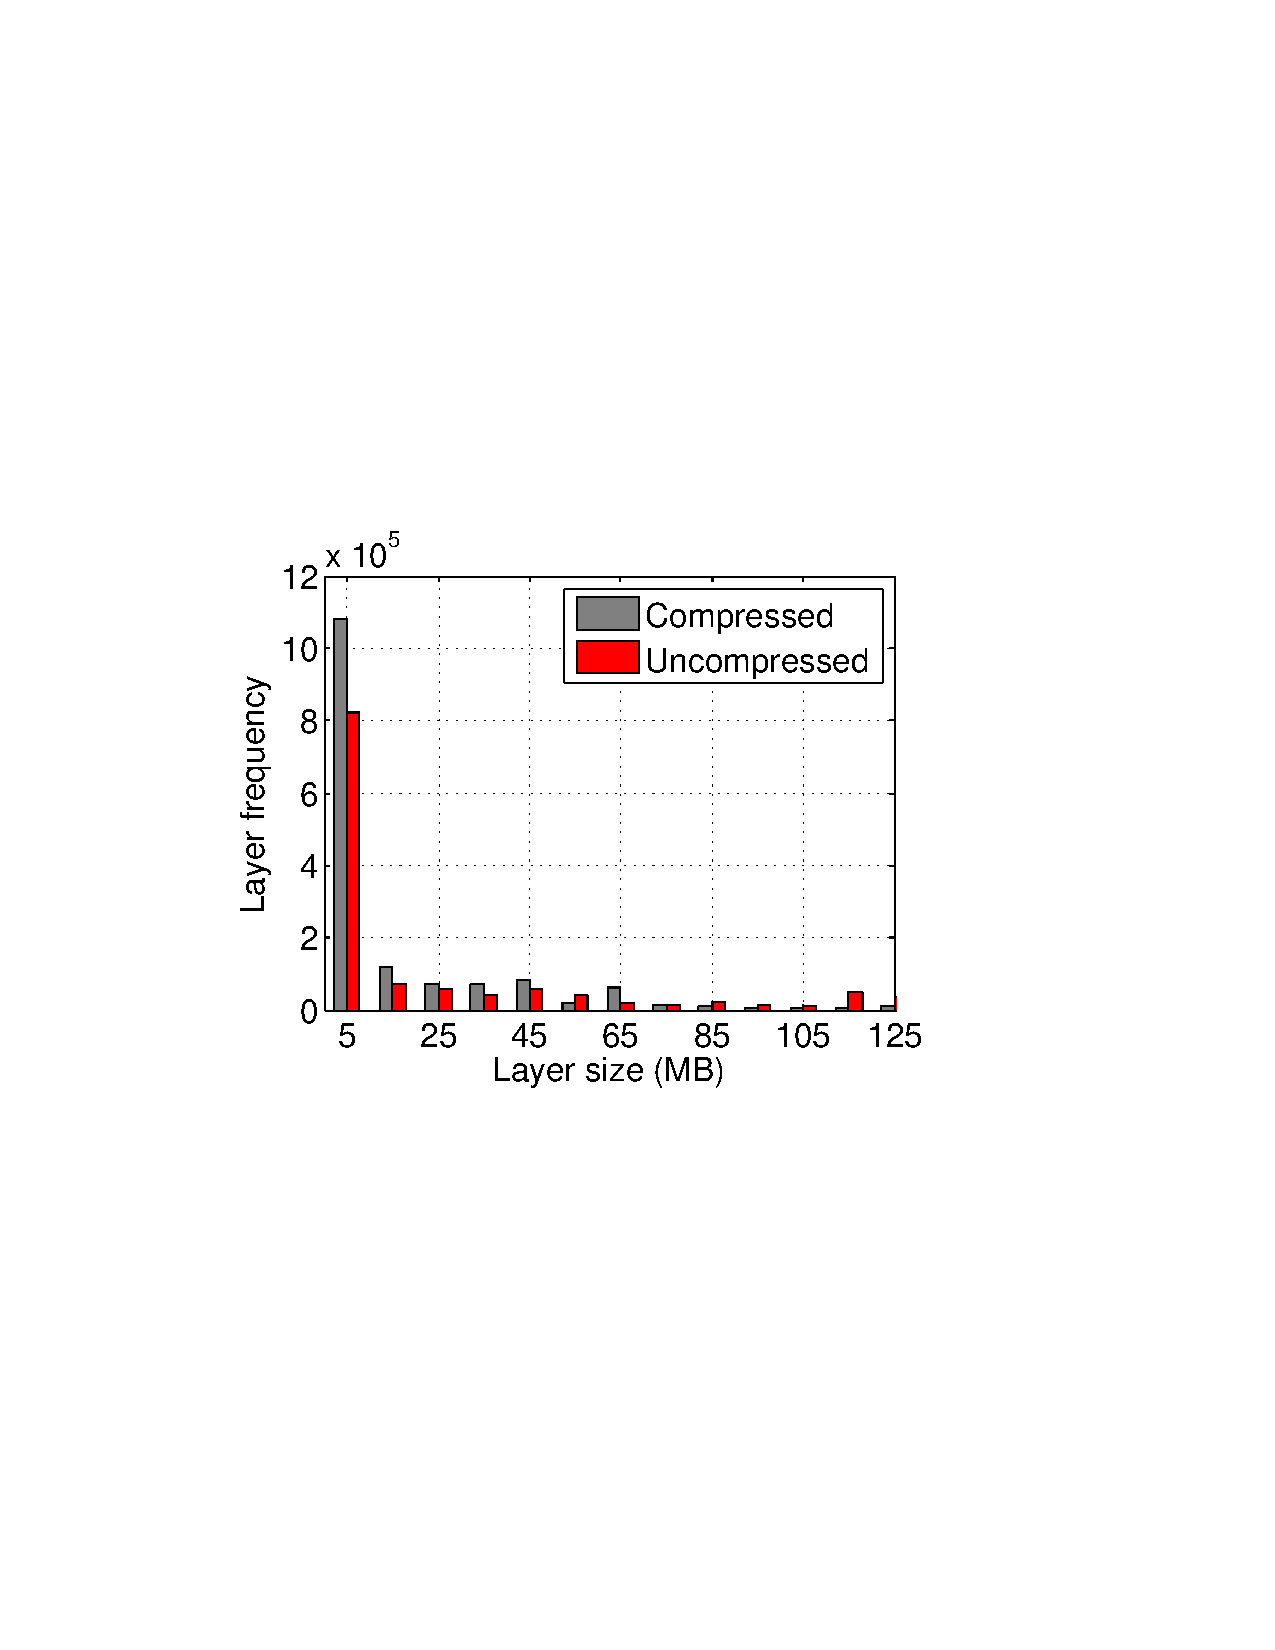
\includegraphics[width=0.213\textwidth]{graphs/hist_layer_size.pdf}
	}
	\caption{Layer size distribution
	\vcomment{Let's use CLS, ALS, and FLS abreviations\nancomment{addressed}}.
	\vcomment{CLS size should go first}.
	\vcomment{We need to use different types of lines (solid, dotted, etc.)
		or markers (round, triangular)}.
	\vcomment{In figure B it is not clear to which bar group corresponds
		  to which layer size. I suggest to try to rotate the graph
		  by 90 grads to fit all layer size labels.\nancomment{aligned label with bar}}
	}
	\label{fig-layer-size}
\end{figure}


We found that most layers'compression ratio is really lower (?) while most of layers have a smaller size. 
So how about we use archiving instead of compression if the network speed is higher (?GB/s)?

\paragraph{Network transfer speed is high!}

\subsubsection{File-level content addressable storage for cold layers}

\paragraph{Image \&. layer popularity skewness} 

\begin{figure}[!t]
	\centering
	\subfigure[CDF of repositories by pull count]{\label{fig_pull_cnt_total}
		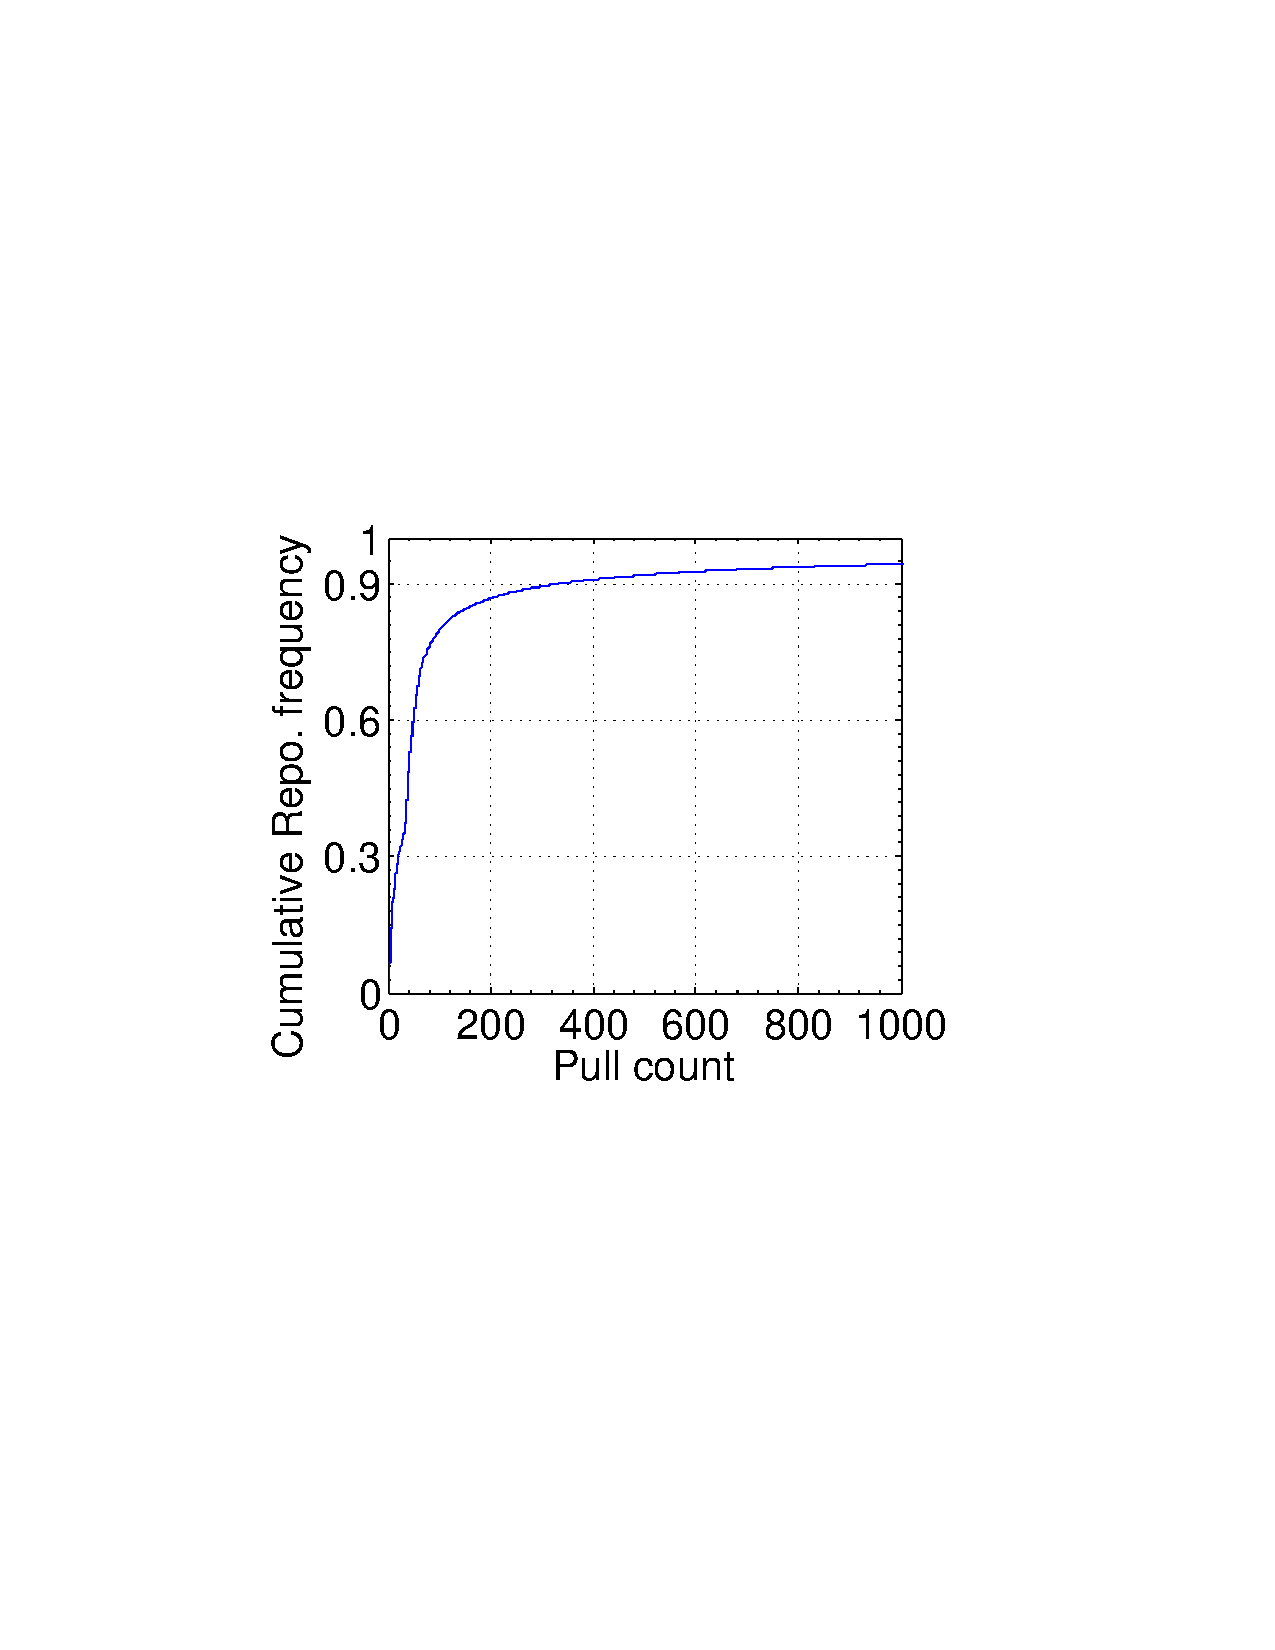
\includegraphics[width=0.23\textwidth]{graphs/pull_cnt.pdf}%
	}
	\subfigure[Histogram of repositories by pull count]{\label{fig_pull_cnt_count}
		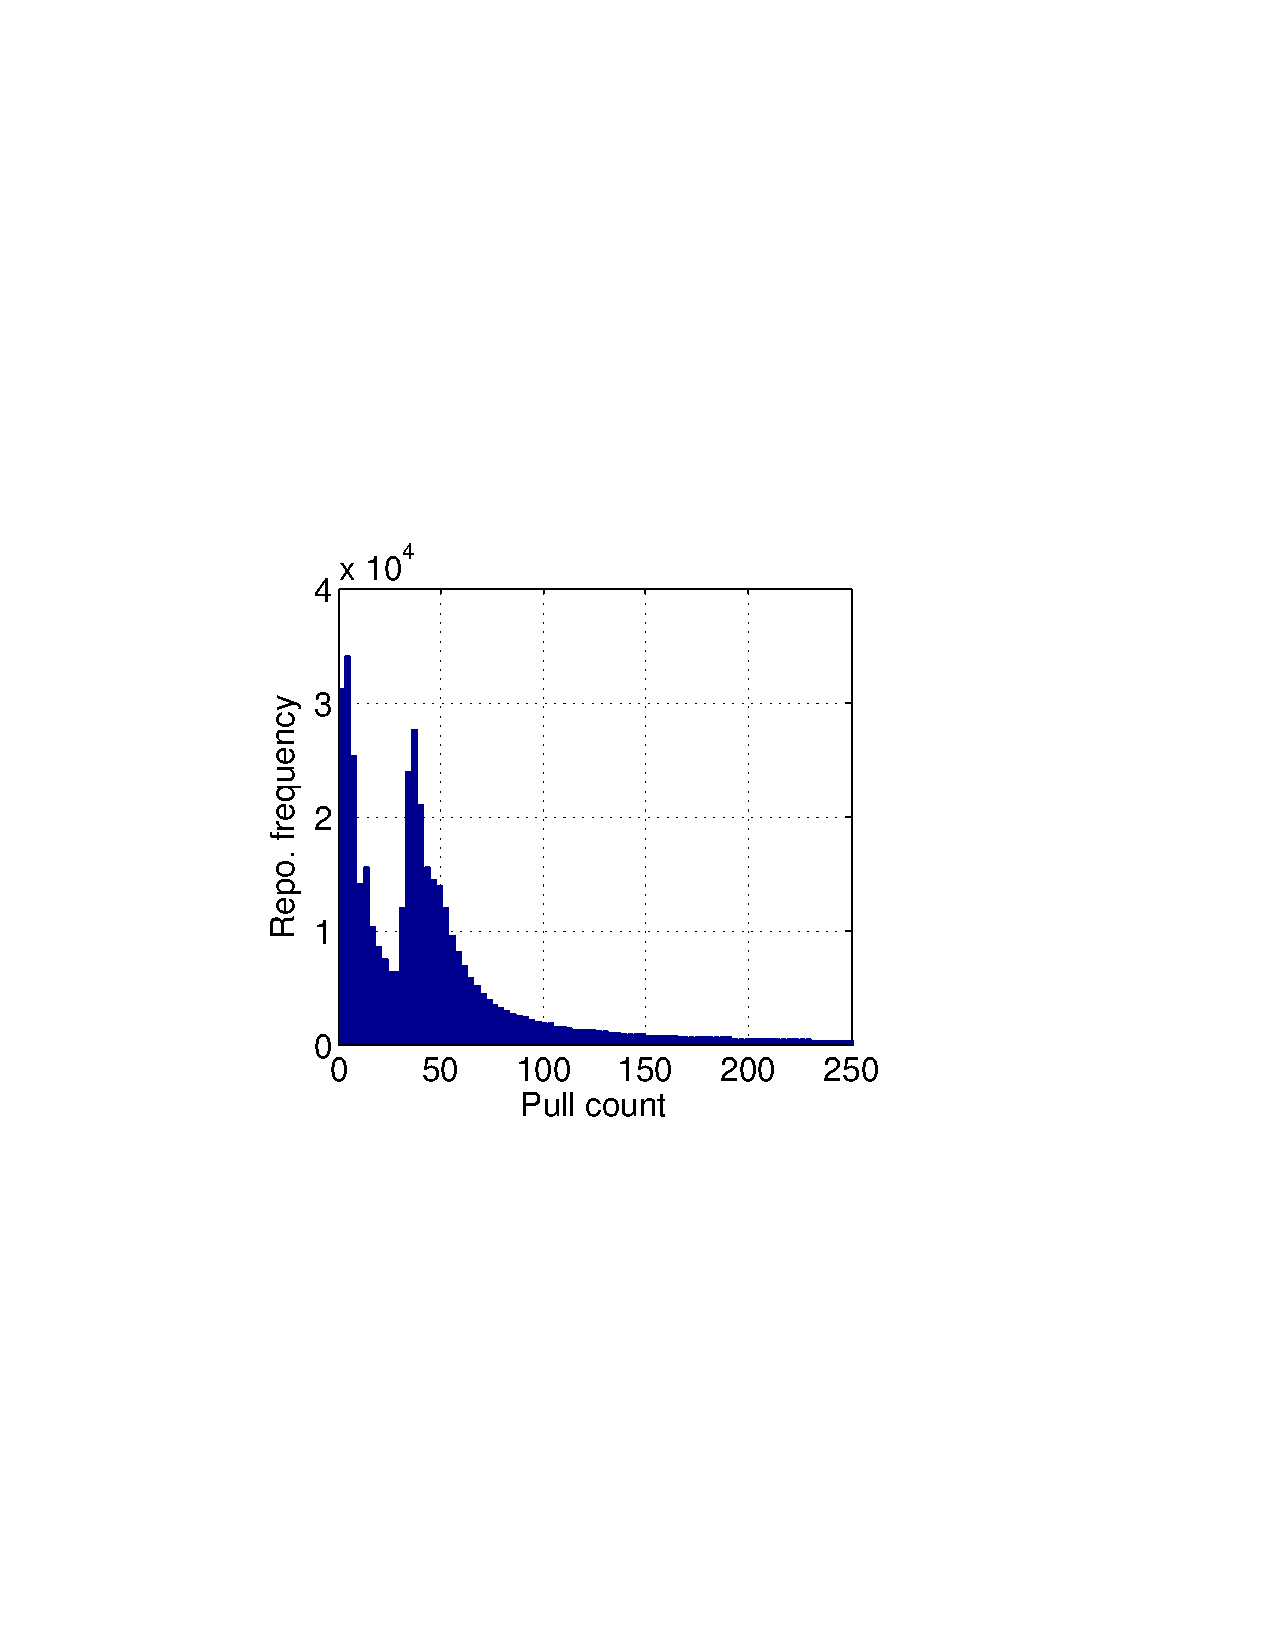
\includegraphics[width=0.22\textwidth]{graphs/count_pull_cnt.pdf}
	}
	\caption{Repository popularity distribution}
	\label{fig-pop}
\end{figure}

\begin{table} 
	\centering 
	\scriptsize  
	%\begin{minipage}{.5\linewidth}
	\caption{Summary of layer \& image characterization} \label{tbl:redundant_ratio} 
	\begin{tabular}{|l|l|l|l|l|}%p{0.14\textwidth} 
		\hline 
		% after \\: \hline or \cline{col1-col2} \cline{col3-col4} ... 
		% after \\: \hline or \cline{col1-col2} \cline{col3-col4} ... 
		Metrics & max & min & median & avg.\\
		\hline
		Compressed layer size &   &   &   &  \\
		\hline
		Uncompressed layer size &   &   &    &  \\
		\hline
		Archival size &  &  & & \\
		\hline
		Compression ratio &   &   &    &  \\
		\hline
		Layer pull cnt. &  &  & & \\
		\hline
		File cnt. per layer &  &  & & \\
		\hline
		Dir. cnt. per layer &  &  & & \\
		\hline
		Layer depth &  &  & & \\
		\hline
		\hline
		Compressed image size &  &  & & \\
		\hline
		Uncompressed image size & &  &  & \\
		\hline
		Archival image size & &  &  & \\
		\hline
		Compression ratio &   &   &    &  \\
		\hline
		Image pull cnt.  &  &  & & \\
		\hline
		Layer cnt. per image  &  &  & & \\
		\hline
		Shared layer cnt. per image  &  &  & & \\
		\hline
		File cnt. per layer &  &  & & \\
		\hline
		Dir. cnt. per layer &  &  & & \\
		\hline	
	\end{tabular} 
\end{table} 

\subsubsection{Constructing shared layers for redundant directories/files}

\paragraph{Smaller number of layers are shared among different images}
\begin{figure}[!t]
	\centering
	\subfigure[CDF of layer reference count]{\label{fig_repeate_layer}
		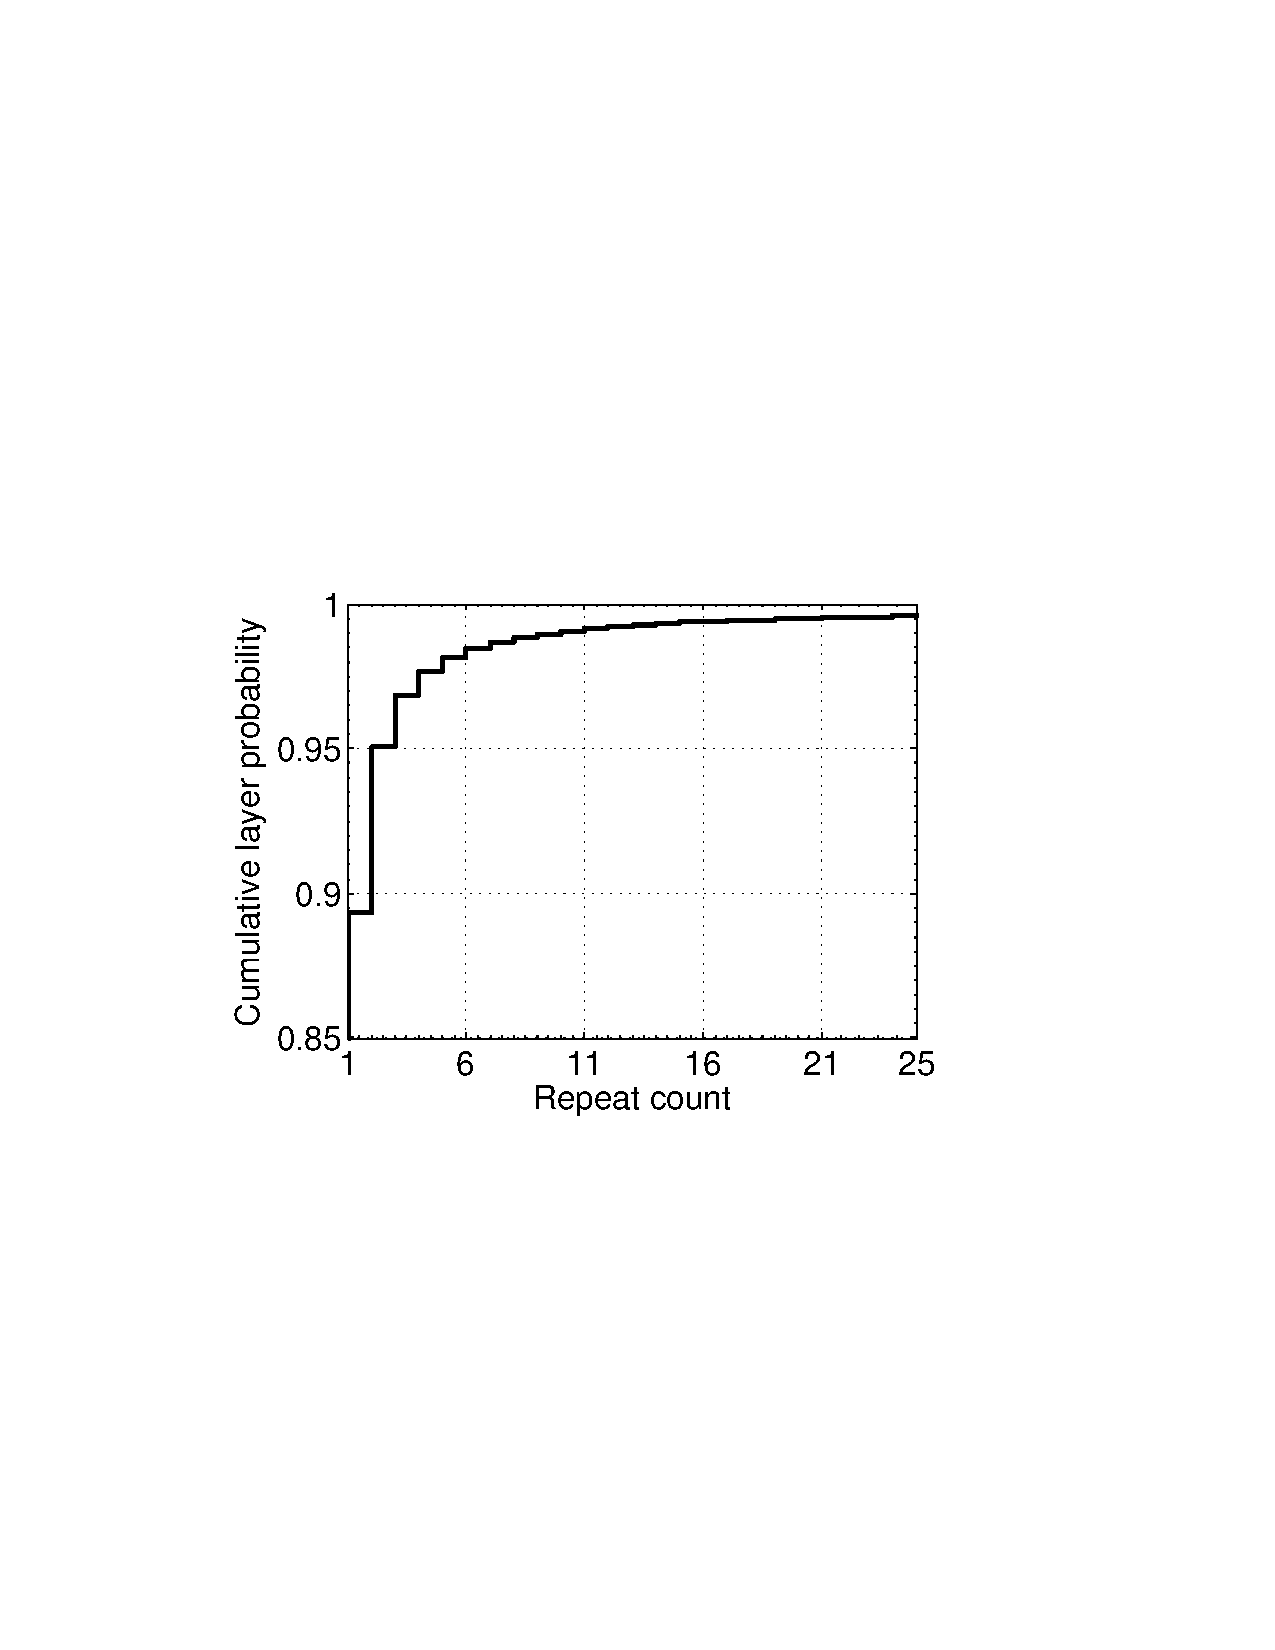
\includegraphics[width=0.23\textwidth]{graphs/repeate_layer.pdf}
	}
	\subfigure[Histogram of layer reference count]{\label{fig_hist_repeate_layer}
		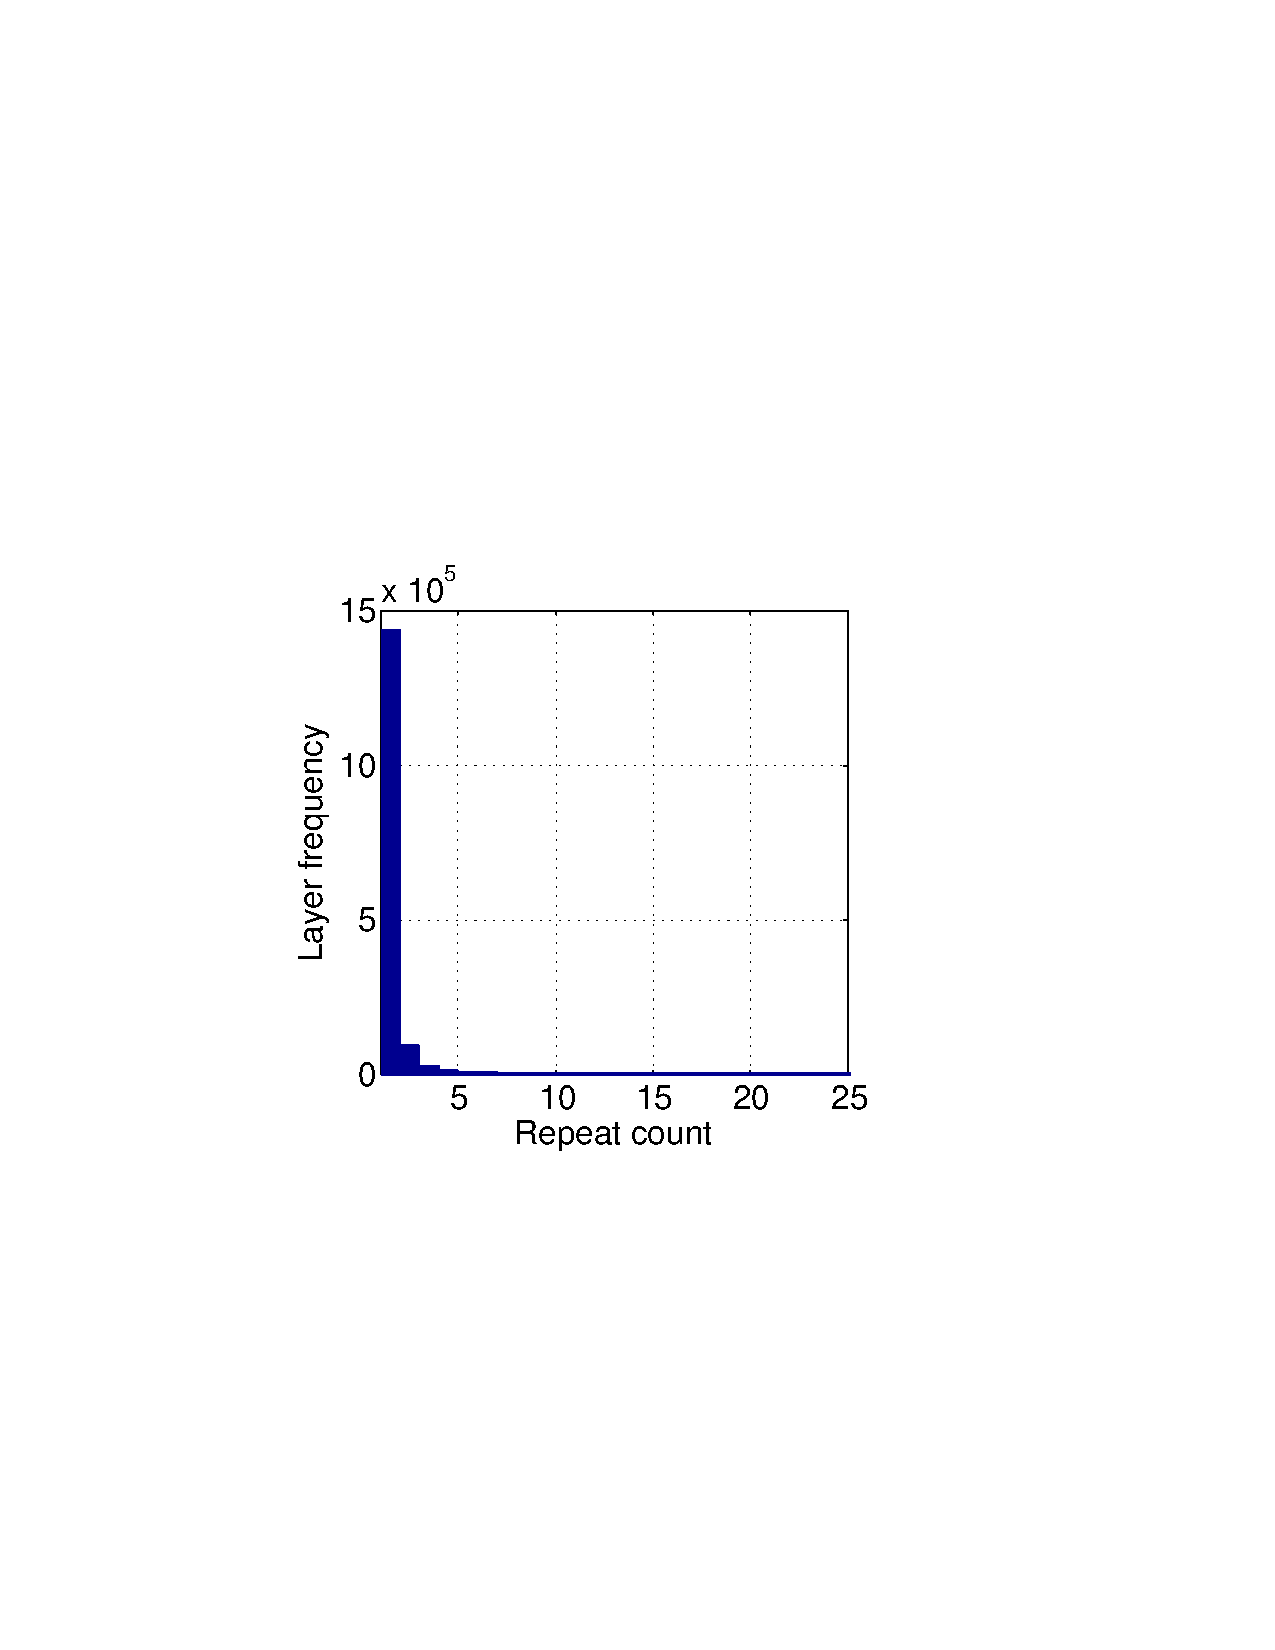
\includegraphics[width=0.223\textwidth]{graphs/hist_repeate_layer.pdf}
	}
	\caption{Layer reference counts across all images}
	\label{fig-repeat-layer-cnt}
\end{figure}

\paragraph{Smaller pull latency than recompression model} the registry can prepare the reconstructed layers before users issue a pull request. But this model requires users to rebuild two layers.

\subsubsection{Summary of Suggestions/trade-offs between dedup ratio and recompression overhead}

\paragraph{1. using archiving instead of compression}
\paragraph{2. using file-level dedup for cold images/layers}
\paragraph{3. using file-level dedup economically}
When to trigger file-level dedup?
\paragraph{4. constructing shared layers for redundant dirs/files, for example,}
%\subsection{Layer reconstruction model}
%\subsubsection{Reconstruction overhead}
%\subsubsection{Trade-offs between dedup ratio and reconstruction overhead}
%\paragraph{Dedup ratio VS. Rebuild overhead}
%\subsection{Evaluation results}